\section{РАЗРАБОТКА ПРОГРАММНОГО КОМПЛЕКСА}

\subsection{Общая архитектура решения}

Разработанная система представляет собой программный комплекс анализа детских рисунков, функционально декомпозированный на пять последовательных модулей в нотации IDEF0~\cite{idef0}. Каждый модуль решает свою подзадачу и передаёт результат следующему этапу обработки. Структура декомпозиции приведена на рисунке~\ref{fig:func-decomposition}.

\begin{figure}[h]
    \centering
    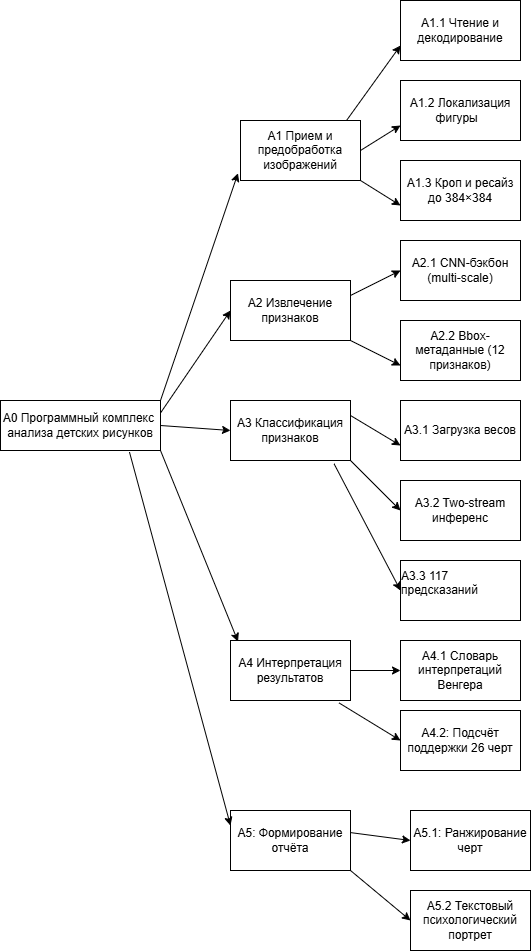
\includegraphics[width=\linewidth,height=0.55\textheight,keepaspectratio]{inc/vkr2.drawio.png}
    \caption{Функциональная декомпозиция программного комплекса анализа детских рисунков}
    \label{fig:func-decomposition}
\end{figure}

Назначение каждого модуля следующее:

\begin{itemize}
    \item A1. Приём и предобработка изображений --- принимает исходный отсканированный рисунок и подготавливает его для нейросетевой модели: чтение и декодирование файла (A1.1), локализация фигуры на основе классических методов обработки изображений (A1.2), кроп и ресайз выделенной области до размера $384 \times 384$ (A1.3);
    \item A2. Извлечение признаков --- формирует входы для нейросетевой модели: визуальные признаки кропа через свёрточный бэкбон (A2.1) и вектор bbox-метаданных из 12 геометрических характеристик (A2.2);
    \item A3. Классификация признаков --- ядро системы. Загружает веса обученной модели (A3.1), выполняет двухпотоковый инференс (A3.2) и формирует 117 предсказаний (A3.3);
    \item A4. Интерпретация результатов --- транслирует предсказания модели в психологические термины с использованием словаря, построенного на основе методики А.~Л.~Венгера (A4.1), и подсчитывает поддержку для каждой из 26 канонических черт (A4.2);
    \item A5. Формирование отчёта --- ранжирует психологические черты по числу подтверждающих признаков (A5.1) и собирает связный текстовый портрет с пояснениями (A5.2).
\end{itemize}

Каждый модуль имеет чётко определённые входы и выходы, что обеспечивает прозрачность работы системы и возможность независимой замены отдельных компонентов. На уровне реализации каждый функциональный модуль вынесен в отдельный микросервис, поверх которых построен веб-интерфейс пользователя (см.~подразделы~2.8--2.13).

\subsection{Описание датасета и его подготовка}

В работе использован датасет из 8179 отсканированных детских рисунков, полученный из образовательных учреждений Самарской области, Республики Чувашии, Московской и Вологодской областей. База изображений и разметка предоставлены Московским государственным психолого-педагогическим университетом, разметка выполнена специалистами в области детской психологии. Сопровождающая CSV-таблица содержит для каждой записи значения 117 экспертно проставленных признаков и служебные поля.

В разметке для 61 уникального кода имеется по нескольку записей с возможными расхождениями значений признаков, что объясняется независимой разметкой одного и того же рисунка несколькими экспертами. Для устранения противоречий применяется голосование большинством (majority vote) по каждому признаку независимо. После дедупликации каждому уникальному коду соответствует одна запись с консолидированной разметкой, записи без соответствующего изображения исключаются. В результате получается выборка из более 7000 примеров.

Для разбиения на обучающую, валидационную и тестовую части применяется групповое стратифицированное разбиение в пропорции 70\,/\,15\,/\,15 с использованием библиотеки iterative-stratification~\cite{iterstrat}. Стратификация выполняется по бинарным индикаторам редких классов наиболее сложных признаков. После дедупликации каждый код встречается ровно один раз, поэтому разбиение автоматически group-safe.

\subsection{Модуль предобработки изображений}

Модуль реализует локализацию фигуры человека на отсканированном листе и формирует кропированное квадратное изображение фиксированного размера и вектор из 12 геометрических метаданных. Алгоритм собран из классических операций библиотеки OpenCV~\cite{opencv} без использования предобученных нейронных моделей детекции, что обеспечивает прозрачность и воспроизводимость поведения модуля.

Конвейер обработки состоит из нескольких этапов. К исходному изображению, приведённому к одноканальному виду, применяется адаптивная бинаризация с гауссовым ядром, выбранная вместо глобального порога из-за неравномерной яркости сканов, затем медианная фильтрация и морфологическое замыкание для объединения близко расположенных штрихов одной фигуры в связную область. Далее с помощью \texttt{cv2.connectedComponentsWithStats} выделяются связные компоненты, каждая из которых проходит проверку по четырём независимым критериям: минимальная площадь, занимаемая доля листа, отношение сторон, плотность заполнения.

Из оставшихся кандидатов выбирается компонента с наибольшей площадью --- якорная, к ней присоединяются все остальные кандидаты, чьи центры масс находятся в пределах адаптивного радиуса. Результирующий ограничивающий прямоугольник расширяется на 8\,\% по каждой стороне, по нему выполняется обрезка, дополнение белым фоном до квадрата и приведение к разрешению $384 \times 384$ билинейной интерполяцией.

Помимо кропа, для каждого изображения вычисляется вектор из 12 геометрических метаданных: относительные ширина, высота, площадь и координаты центра bbox; отношение высоты к ширине; четыре бинарных индикатора касания краёв листа; нормализованное расстояние от центра bbox до ближайшего угла; индикатор источника детекции. Эти метаданные используются как второй вход нейронной сети (см.~подраздел~2.4) и сохраняют информацию о размере и положении фигуры на исходном листе, утрачиваемую после кропа.

\subsection{Архитектура нейросетевой модели}

Для классификации 117 признаков спроектирована двухпотоковая свёрточная нейронная сеть, обучаемая полностью с нуля на целевой выборке детских рисунков. Общая схема архитектуры приведена в приложении на рисунке~\ref{fig:drawingnet-arch-appendix}.

Выбор обучения с нуля вместо transfer learning с предобученным бэкбоном (например, ResNet-50) мотивирован существенным отличием статистики детских карандашных рисунков от естественных фотоизображений ImageNet. ImageNet-предобучение оптимизирует свёрточные ядра под детектирование цветных текстур и градиентов яркости, в то время как карандашный рисунок представляет собой набор тёмных линий на однородном светлом фоне. В предварительных экспериментах модели на основе предобученного ResNet-50/152 не давали статистически значимого выигрыша по F1-мере над моделью, обученной с нуля, при существенно большем числе параметров (около 60 млн против 5,5 млн у разработанной модели).

Первый поток обрабатывает кропированное изображение размером $320 \times 320$ пикселей. Уменьшение разрешения с $384$ до $320$ выполнено для сокращения объёма вычислений на инференсе без существенной потери качества (потеря F1 в предварительных экспериментах --- около 0,003). Сеть состоит из пяти этапов:

\begin{itemize}
    \item Stem --- первый свёрточный слой с ядром $7 \times 7$, BatchNorm~\cite{batchnorm}, ReLU и max-pool $3 \times 3$ со страйдом 2. Большое начальное ядро мотивировано особенностью детских рисунков: типичные карандашные штрихи длинные, и одно ядро $7 \times 7$ захватывает целые сегменты, в отличие от стандартных ядер $3 \times 3$ современных backbone'ов;
    \item Stage~2 (64 канала) --- два residual-блока с последующим max-pool;
    \item Stage~3 (128 каналов) --- два residual-блока с последующим max-pool;
    \item Stage~4 (256 каналов) --- два residual-блока с последующим max-pool, выход используется как первый источник многомасштабных признаков;
    \item Stage~5 (384 канала) --- один residual-блок, выход используется как второй источник многомасштабных признаков.
\end{itemize}

Каждый residual-блок реализует стандартную схему с двумя свёртками $3 \times 3$, BatchNorm и ReLU и пропускающим (skip) соединением. При несовпадении числа каналов или страйда в skip-соединение добавляется проекционная свёртка $1 \times 1$. Использование residual-связей обеспечивает устойчивое распространение градиентов в глубокой сети и облегчает оптимизацию~\cite{resnet}.

С целью повышения детализации признакового представления используется конкатенация выходов четвёртого и пятого этапов, пропущенных через адаптивный усредняющий пулинг до размера $1 \times 1$:
\begin{equation}
\mathbf{f}_{img} = \left[\, \text{pool}(\text{stage}_4(x))\ ;\ \text{pool}(\text{stage}_5(x)) \,\right] \in \mathbb{R}^{640}
\end{equation}

Применение конкатенации признаков с двух уровней обусловлено следующими соображениями. Признаки stage~4 (256 каналов) содержат среднеуровневые геометрические паттерны (формы, очертания, локальные особенности), полезные для распознавания мелких деталей рисунка (форма глаз, наличие пуговиц, штриховка). Признаки stage~5 (384 канала) содержат высокоуровневые семантические признаки, релевантные для общих характеристик (поза фигуры, ракурс, размер). Совместное использование обоих уровней даёт богатое признаковое представление, способное обслуживать как мелкозернистые, так и крупнозернистые задачи распознавания.

Второй поток обрабатывает 12-мерный вектор геометрических метаданных, выработанных модулем предобработки. Перед подачей в сеть метаданные нормируются по среднему и стандартному отклонению, вычисленным на обучающей выборке. Преобразование выполняет двухслойный MLP с активациями ReLU и одним слоем дропаута~\cite{dropout}:
\begin{equation}
\mathbf{f}_{bbox} = \text{MLP}(\mathbf{x}_{bbox}) \in \mathbb{R}^{64}
\end{equation}

Необходимость второго потока обусловлена тем, что после кропа и ресайза фигуры к фиксированному размеру в визуальном представлении теряется информация о её абсолютном размере и положении на исходном листе. Между тем эта информация существенна для ряда признаков рисуночного теста: <<размер рисунка>> определяется отношением площади фигуры к площади листа, <<расположение>> и <<смещение>> --- координатами центра фигуры на странице, признак <<обрезано>> --- касанием bbox-фигуры краёв листа.

Векторы признаков от двух потоков конкатенируются и пропускаются через одну из двух параллельных проекционных голов. Признаки, для которых ожидается повышенная сложность распознавания, направляются через выделенную проекцию; остальные --- через общую проекцию. Такое разделение --- разновидность многозадачного обучения с группировкой задач~\cite{multitask-survey} --- уменьшает конкуренцию градиентов между задачами разной сложности и обеспечивает более устойчивое обучение признаков с малым числом примеров. Каждая проекция сужает признаковое пространство до 256 нейронов с дропаутом 0,3.

Финальный слой состоит из 117 параллельных классификационных голов: каждая голова --- один линейный слой, отображающий 256-мерный признак в логиты соответствующего числа классов (2 для бинарного признака, $K$ для категориального с $K$ классами). Все 117 голов организованы в виде \texttt{nn.ModuleDict}, что обеспечивает прозрачную адресацию к голове по имени критерия и упрощает сохранение и загрузку модели.

Общее число параметров модели составляет около 5,5~миллионов, размер сохранённого чекпоинта --- около 22~МБ. Инициализация всех свёрточных и линейных слоёв выполнена методом Кайминга~\cite{kaiming-init}, что соответствует выбранной активации ReLU и обеспечивает корректное масштабирование начальных активаций по слоям. На рисунке~\ref{src:src3} представлен фрагмент реализации определения архитектуры модели и процедуры обучения.

\begin{figure}
    \lstinputlisting[language=Python]{inc/code2.py}
    \caption{Фрагмент кода реализации обучения}
    \label{src:src3}
\end{figure}

\subsection{Функции потерь и стратегия обучения}

Для бинарного признака используется взвешенная перекрёстная энтропия с весами классов $\alpha = (1.0,\ \min(\sqrt{N_-/N_+},\ 10))$, где $N_\pm$ --- количества отрицательных и положительных примеров. Корень из отношения и ограничение значением 10 защищают градиент от взрыва при экстремальном дисбалансе. В качестве альтернативы рассматривалась фокальная функция потерь~\cite{focal-loss}, однако сочетание корневого взвешивания и WeightedRandomSampler даёт сопоставимое поведение при меньшем числе гиперпараметров для подбора.

Для категориального признака используется взвешенная перекрёстная энтропия с label smoothing $0.05$ и весами $\alpha_i = \min(\sqrt{N_{max}/N_i},\ 10)$. Совокупная функция потерь --- среднее по 117 признакам:
\begin{equation}
\mathcal{L} = \frac{1}{117} \sum_{i=1}^{117} \mathcal{L}_i(\mathbf{f}_{proj},\ y_i)
\end{equation}

Дополнительно применяется WeightedRandomSampler: каждому примеру обучающей выборки присваивается вес, повышенный относительно базового для тех примеров, которые имеют положительные метки редких классов. Веса ограничены диапазоном $[1, 2.5]$, сэмплирование выполняется с возвращением. На рисунке~\ref{src:src4} приведён фрагмент реализации цикла обучения с вычислением функций потерь и обновлением параметров модели.

\begin{figure}
    \lstinputlisting[language=Python]{inc/code3.py}
    \caption{Фрагмент кода реализации цикла обучения}
    \label{src:src4}
\end{figure}

К каждому изображению применяется набор аугментаций: random affine ($\pm6^\circ$, сдвиг до 5\,\%, масштаб 90--110\,\%), random crop из увеличенного на 32~пикселя изображения до $320\times320$, color jitter (яркость и контраст до 15\,\%), random erasing с вероятностью 0,2. Намеренно не используется горизонтальное отражение, поскольку ряд признаков содержит указание на правую и левую стороны.

Оптимизатор --- AdamW~\cite{adamw,adam} с базовой скоростью обучения $10^{-4}$, weight decay $5 \cdot 10^{-4}$, обрезкой нормы градиента до 1,0. Размер пакета --- 32. Расписание LR --- косинусное затухание с разогревом в течение трёх эпох~\cite{cosine-schedule}. Смешанная точность намеренно отключена в пользу одинарной (fp32): при обучении с нуля и сильных весовых коэффициентах функции потерь начальные градиенты могут принимать большие значения, и в режиме fp16 это иногда приводит к численным переполнениям. Полное число эпох --- 50 с ранней остановкой по отсутствию улучшения F1 на валидации в течение 8 эпох с минимумом в 25 эпох.

\subsection{Словарь интерпретаций признаков}

Связь между техническими признаками рисунка и психологическими чертами реализована через JSON-словарь \texttt{criteria\_interpretations.json} объёмом около 60~КБ. Структура словаря: раздел \texttt{traits} --- 26 канонических черт с текстовыми описаниями; раздел \texttt{criteria} --- 117 признаков с указанием типа, набора связанных черт; раздел \texttt{meta} --- сведения о версии и источниках. Содержательная составляющая построена на основе книги А.~Л.~Венгера~\cite{venger}.

Один признак может быть индикатором нескольких черт, а одна черта обычно поддерживается набором различных признаков. При использовании словаря в составе генератора портрета каждой черте сопоставляется счётчик поддержки, равный количеству предсказанных моделью признаков, ассоциированных с ней. Это позволяет ранжировать черты в итоговом тексте по степени их выраженности. В таблице~\ref{traits-list} приведена часть канонических черт.

\begin{table}
    \caption{Часть канонических психологических черт}
    \fontsize{12pt}{14pt}\selectfont
    \begin{tabular}{|p{60mm}|p{90mm}|}\hline
        \textbf{Черта} & \textbf{Краткое пояснение} \\ \hline
        Тревожность личностная           & Устойчивая склонность к беспокойству, сниженная самооценка \\ \hline
        Состояние тревоги                & Ситуативная тревога, проявленная в момент рисования \\ \hline
        Демонстративность                & Стремление быть в центре внимания, экспансивное поведение \\ \hline
        Агрессивность                    & Склонность к враждебному, конкурентному поведению \\ \hline
    \end{tabular}
    \label{traits-list}
\end{table}

\subsection{Генератор текстового психологического портрета}

Модуль принимает на вход словарь предсказаний модели $\{c_i \mapsto v_i\}_{i=1}^{117}$ и словарь интерпретаций. Для каждого признака с положительным предсказанием ($v_i \neq 0,\ v_i \neq \text{пусто}$) извлекается соответствующий список черт, и для каждой черты $t$ инкрементируется счётчик поддержки:
\begin{equation}
S(t) = \sum_{i=1}^{117} \mathbb{1}\big[\, t \in \text{traits}(c_i, v_i) \,\big]
\end{equation}
Параллельно для каждой черты накапливается список свидетельств --- пар <<признак, значение>>, давших вклад в её поддержку.

Финальный текст портрета содержит заголовок и краткое пояснение, перечень из 7 наиболее устойчиво проявленных черт с порогом поддержки не менее 2 признаков --- для каждой приводится описание и до 4 подтверждающих свидетельств, --- раздел менее устойчивых тенденций с поддержкой 1 признака и итоговое замечание о вероятностном характере выводов. Объём типового портрета --- 25--40 строк. На рисунке~\ref{src:src5} представлен фрагмент кода, реализующий логику формирования психологического портрета на основе предсказаний модели и словаря интерпретаций.

\begin{figure}
    \lstinputlisting[language=Python]{inc/code4.py}
    \caption{Фрагмент кода для генерации психологического портрета}
    \label{src:src5}
\end{figure}

\subsection{Микросервисная архитектура веб-сервиса}

Программный комплекс реализован в виде микросервисного веб-приложения, архитектура которого представлена на рисунке~\ref{fig:veb-arch}. Система разделена на три логических контура, объединённых единым API-шлюзом.

\begin{figure}
    \centering
    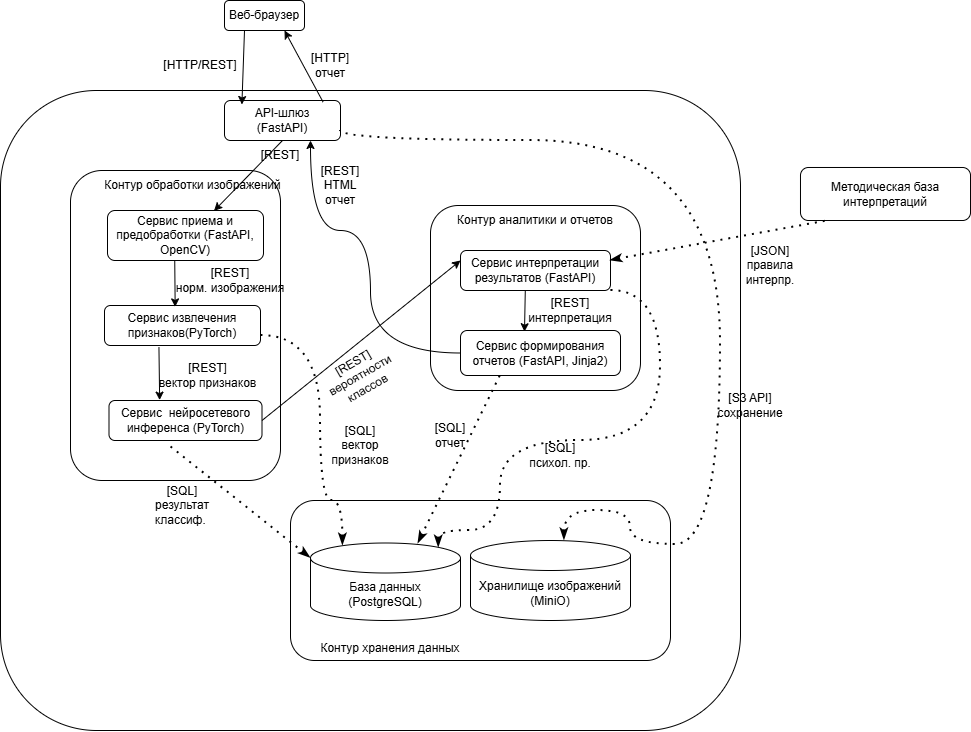
\includegraphics[width=\linewidth,height=0.6\textheight,keepaspectratio]{inc/veb-arch.png}
    \caption{Архитектура веб-сервиса: микросервисы, протоколы взаимодействия и контуры хранения данных}
    \label{fig:veb-arch}
\end{figure}

API-шлюз (FastAPI~\cite{fastapi}) --- единственная точка входа для внешнего пользователя. Принимает HTTP/REST-запросы от веб-браузера, оркестрирует последовательные вызовы к внутренним сервисам и возвращает итоговый HTML-отчёт. Шлюз также отвечает за сохранение изображений в объектное хранилище MinIO~\cite{minio} (S3 API) и метаданных анализа в реляционную базу PostgreSQL~\cite{postgres}.

Контур обработки изображений включает три сервиса, образующих последовательный конвейер:

\begin{enumerate}
    \item сервис приёма и предобработки (FastAPI~\cite{fastapi}, OpenCV~\cite{opencv}) --- принимает исходное изображение, выполняет локализацию фигуры и возвращает нормализованное изображение и координаты bbox;
    \item сервис извлечения признаков (FastAPI~\cite{fastapi}) --- вычисляет 12-мерный вектор геометрических метаданных на основе координат bbox;
    \item сервис нейросетевого инференса (PyTorch~\cite{pytorch}) --- загружает обученную модель и выполняет классификацию: принимает изображение и вектор признаков, возвращает вероятности 117~классов.
\end{enumerate}

Между сервисами контура данные передаются по REST: нормализованное изображение и вектор признаков последовательно проходят через конвейер. Результат классификации в виде вероятностей классов передаётся в следующий контур.

Контур аналитики и отчётов включает два сервиса:

\begin{enumerate}
    \item сервис интерпретации результатов (FastAPI~\cite{fastapi}) --- принимает вектор вероятностей классов и транслирует его в психологические черты с использованием методической базы интерпретаций (JSON-словарь, построенный по методике А.~Л.~Венгера~\cite{venger});
    \item сервис формирования отчётов (FastAPI~\cite{fastapi}) --- принимает интерпретацию и формирует HTML-документ психологического портрета, который возвращается API-шлюзу.
\end{enumerate}

Контур хранения данных обеспечивает персистентность:

\begin{itemize}
    \item база данных (PostgreSQL~\cite{postgres}) --- хранит метаданные анализов, предсказания модели, поддержку черт и сгенерированные портреты;
    \item хранилище изображений (MinIO~\cite{minio}) --- хранит исходные сканы рисунков и результаты предобработки через S3-совместимый интерфейс.
\end{itemize}

Все внутренние сервисы взаимодействуют по протоколу REST через локальную Docker-сеть~\cite{docker}. Внешний доступ открыт только для API-шлюза (порт 8000); остальные сервисы изолированы от внешних запросов, что снижает поверхность атаки.

Такая архитектура обеспечивает независимое масштабирование отдельных компонентов --- при увеличении нагрузки можно горизонтально масштабировать только сервис инференса, --- технологическую независимость сервисов, отказоустойчивость, при которой сбой одного сервиса не приводит к падению системы, и возможность замены модели без затрагивания остальных компонентов.

Состав сервисов и их порты приведены в таблице~\ref{services-list}.

\begin{table}
    \caption{Состав микросервисов программного комплекса}
    \fontsize{12pt}{14pt}\selectfont
    \begin{tabular}{|p{30mm}|p{15mm}|p{99mm}|}\hline
        \textbf{Сервис} & \textbf{Порт} & \textbf{Назначение} \\ \hline
        api-gateway      & 8000  & Веб-интерфейс, оркестрация цепочки, сохранение результата в БД и MinIO \\ \hline
        preprocessing    & 8001  & Локализация фигуры (OpenCV~\cite{opencv} + YOLO-резерв~\cite{yolov8}), кроп и ресайз до $384 \times 384$ \\ \hline
        features         & 8002  & Вычисление 12 геометрических bbox-признаков \\ \hline
        inference        & 8003  & Нейросетевой инференс: $\text{(image, bbox)} \mapsto 117$ предсказаний \\ \hline
        interpretation   & 8004  & Маппинг 117 предсказаний $\rightarrow$ 26 психологических черт \\ \hline
        report           & 8005  & Рендер HTML-портрета по шаблону Jinja2 \\ \hline
    \end{tabular}
    \label{services-list}
\end{table}

\subsection{Технологический стек}

В качестве основного языка разработки выбран Python~3.11 ввиду того, что обученная нейросетевая модель и алгоритмы предобработки изображений уже реализованы на этом языке. Для построения REST-сервисов используется фреймворк FastAPI~\cite{fastapi} с автоматической генерацией OpenAPI-схемы и валидацией входных данных через Pydantic. ASGI-сервер --- Uvicorn~\cite{uvicorn}.

Сервис инференса использует библиотеку PyTorch~\cite{pytorch} для загрузки и выполнения нейросетевой модели, сервис предобработки --- библиотеки OpenCV~\cite{opencv} (адаптивная бинаризация, морфология, выделение связных компонент) и Ultralytics (резервный YOLOv8-детектор~\cite{yolov8}). Для межсервисного взаимодействия по HTTP используется асинхронный клиент httpx, шаблонизатор для HTML-портретов и веб-интерфейса --- Jinja2.

Сервис \texttt{api-gateway} взаимодействует с внешними системами хранения через стандартизированные клиенты: \texttt{psycopg} (PostgreSQL) и \texttt{minio} (MinIO S3-совместимое объектное хранилище). Все библиотечные зависимости каждого сервиса вынесены в \texttt{requirements.txt} и устанавливаются изолированно при сборке образа.

\subsection{Описание сервисов}

api-gateway --- единственная точка входа для пользователя. Предоставляет HTML-форму загрузки рисунка на главной странице, страницу истории анализов и страницу повторного просмотра сохранённого портрета по его идентификатору. При получении нового запроса сервис генерирует UUID анализа, последовательно вызывает остальные сервисы, сохраняет промежуточные результаты в MinIO, а финальный результат --- в PostgreSQL. HTML-шаблоны (форма загрузки, история, страница ошибки) выполнены на Jinja2.

preprocessing --- реализует алгоритм локализации фигуры из подраздела~2.3. На вход поступает multipart-файл изображения, на выход --- base64-кодированный кроп размером $384 \times 384$, координаты bbox на исходном листе, размеры исходного изображения и индикатор источника детекции. Если основной OpenCV-алгоритм не обнаруживает достаточно крупной связной области, выполняется резервная детекция через YOLOv8 --- готовый детектор людей используется в роли подстраховки, что повышает робастность системы к редким сложным случаям сканирования.

features --- лёгкий вычислительный сервис, принимающий координаты bbox и размеры исходного листа и возвращающий вектор из 12 геометрических признаков, описанных в подразделе~2.3. Сервис не содержит ML-зависимостей, выполняется в считанные миллисекунды и легко горизонтально масштабируется.

inference --- ядро системы. При запуске контейнера загружает веса обученной модели, словари label encoders, а также маски \texttt{target/nontarget}, восстановленные из вспомогательного pickle-файла \texttt{encoders.pkl}. На вход принимает изображение и 12-мерный вектор bbox-фичей; на выход выдаёт словарь 117 предсказаний и сопутствующих confidences (значения softmax по предсказанному классу). Сервис не требует GPU --- инференс выполняется на CPU за порядка 0,2~секунды на одно изображение.

interpretation --- применяет словарь \texttt{criteria\_interpretations.json} к 117 предсказаниям, формирует словарь поддержки 26 черт и список свидетельств (см.~подраздел~2.7). Логика модуля не содержит обучаемых параметров и реализована на чистом Python.

report --- финальный шаг конвейера. Принимает словарь черт, список свидетельств и (опционально) ссылки на изображения в MinIO, формирует HTML-документ психологического портрета по шаблону Jinja2 с применением CSS-стилей. Сгенерированный HTML возвращается обратно \texttt{api-gateway}, который сохраняет его в PostgreSQL и отдаёт пользователю.

\subsection{Хранение данных}

Хранение данных распределено между двумя внешними системами в соответствии с типами хранимых данных.

Реляционная СУБД PostgreSQL~\cite{postgres} версии 16 хранит метаданные анализов: уникальный идентификатор, временную метку, оригинальное имя файла, ключи в объектном хранилище, источник детекции, словарь 117 предсказаний, словарь поддержки 26 черт и сгенерированный HTML-портрет. Структура одной таблицы \texttt{analyses} приведена в приложении. На полях временной метки и источника детекции созданы B-tree индексы для ускорения выборки в истории анализов. Хранение предсказаний и поддержки в виде JSONB позволяет гибко расширять формат без миграций схемы.

Объектное хранилище MinIO~\cite{minio} хранит бинарные файлы --- исходные сканы рисунков и кропы, выработанные модулем предобработки. Ключи объектов имеют структуру \texttt{drawings/\{analysis\_id\}/\{original|cropped\}.png}, что обеспечивает однозначное соответствие между записью в PostgreSQL и связанными с ней файлами. MinIO выбран в качестве замены прямого хранения файлов в файловой системе по нескольким причинам: совместимый с Amazon S3 интерфейс упрощает миграцию в облако; встроенная веб-консоль обеспечивает прямой доступ к содержимому для администратора; разделение бинарных файлов и метаданных согласуется с микросервисной идеологией.

Такое разделение обеспечивает выполнение основного принципа проектирования: метаданные хранятся в РСУБД, где они индексируются и связываются по отношениям, а бинарные файлы --- в объектном хранилище, где их объём не влияет на производительность РСУБД.

\subsection{Контейнеризация и развёртывание}

Все сервисы и системы хранения упакованы в Docker-контейнеры~\cite{docker}; для запуска используется единый файл \texttt{docker-compose.yml}, описывающий граф зависимостей между сервисами, переменные окружения, тома для постоянного хранения данных и проброс портов. Сборка каждого сервиса выполняется из собственного \texttt{Dockerfile} в каталоге \texttt{services/<service-name>/}; общие данные (веса модели, словари) монтируются как read-only том из директории \texttt{shared/data/} в путь \texttt{/data} внутри контейнеров.

В составе \texttt{docker-compose.yml} выделены три логических контура: контур обработки изображений (preprocessing, features, inference), контур аналитики и отчётов (interpretation, report), контур хранения (postgres, minio). Шлюз \texttt{api-gateway} оркестрирует обращения ко всем трём контурам и предоставляет единый внешний интерфейс на порту 8000. Дополнительно описан профиль \texttt{tools}, в котором одноразово запускается утилита \texttt{encoders-builder}, собирающая из исходных CSV-таблиц консолидированный pickle-файл с label encoders для сервиса инференса.

Все сервисы конфигурируются через переменные окружения, перечисленные в файле \texttt{.env}, что позволяет менять конфигурацию (имена базы, пароли, URL внутренних сервисов) без пересборки образов. Для запуска полного стека достаточно одной команды \texttt{docker compose up}, что упрощает развёртывание на новом сервере или локальной машине разработчика.

\subsection{Поток данных при анализе одного рисунка}

При загрузке нового рисунка через веб-интерфейс выполняется следующая последовательность обращений между сервисами:

\begin{enumerate}
    \item \texttt{api-gateway} принимает HTTP POST с файлом изображения, генерирует идентификатор анализа (UUID), сохраняет оригинал в MinIO по ключу \texttt{drawings/\{id\}/original.png};
    \item обращение к \texttt{preprocessing}\,/crop --- модуль возвращает кроп в base64, координаты bbox, размеры исходного изображения и источник детекции;
    \item полученный кроп сохраняется в MinIO по ключу \texttt{drawings/\{id\}/cropped.png};
    \item обращение к \texttt{features}\,/compute с координатами bbox и размерами оригинала --- модуль возвращает вектор из 12 геометрических признаков;
    \item обращение к \texttt{inference}\,/predict с изображением и вектором bbox-фичей --- модуль возвращает 117 предсказаний и их confidences;
    \item обращение к \texttt{interpretation}\,/derive с 117 предсказаниями --- модуль возвращает поддержку 26 черт и список свидетельств;
    \item обращение к \texttt{report}\,/render с данными о чертах и свидетельствами --- модуль возвращает HTML-документ психологического портрета;
    \item \texttt{api-gateway} сохраняет в Postgres метаданные анализа (идентификатор, ключи в MinIO, предсказания, поддержку черт, HTML-портрет) и возвращает HTML пользователю.
\end{enumerate}

Все обращения между сервисами выполняются по локальной docker-сети с использованием доменных имён сервисов (например, \texttt{http://inference:8003/predict}), не выходят за пределы хоста и не предполагают аутентификации. Пользовательский интерфейс взаимодействует только с \texttt{api-gateway} через порт 8000.

Сохранённый результат доступен в дальнейшем через раздел истории анализов и может быть открыт повторно по идентификатору без выполнения цепочки заново --- сохранённый HTML-портрет извлекается из PostgreSQL и отдаётся пользователю без обращения к остальным сервисам. Это обеспечивает быстрый просмотр уже выполненных анализов и снижает нагрузку на сервис инференса.
